\chapter{The Activation}
\label{ch:22}



\begin{center}
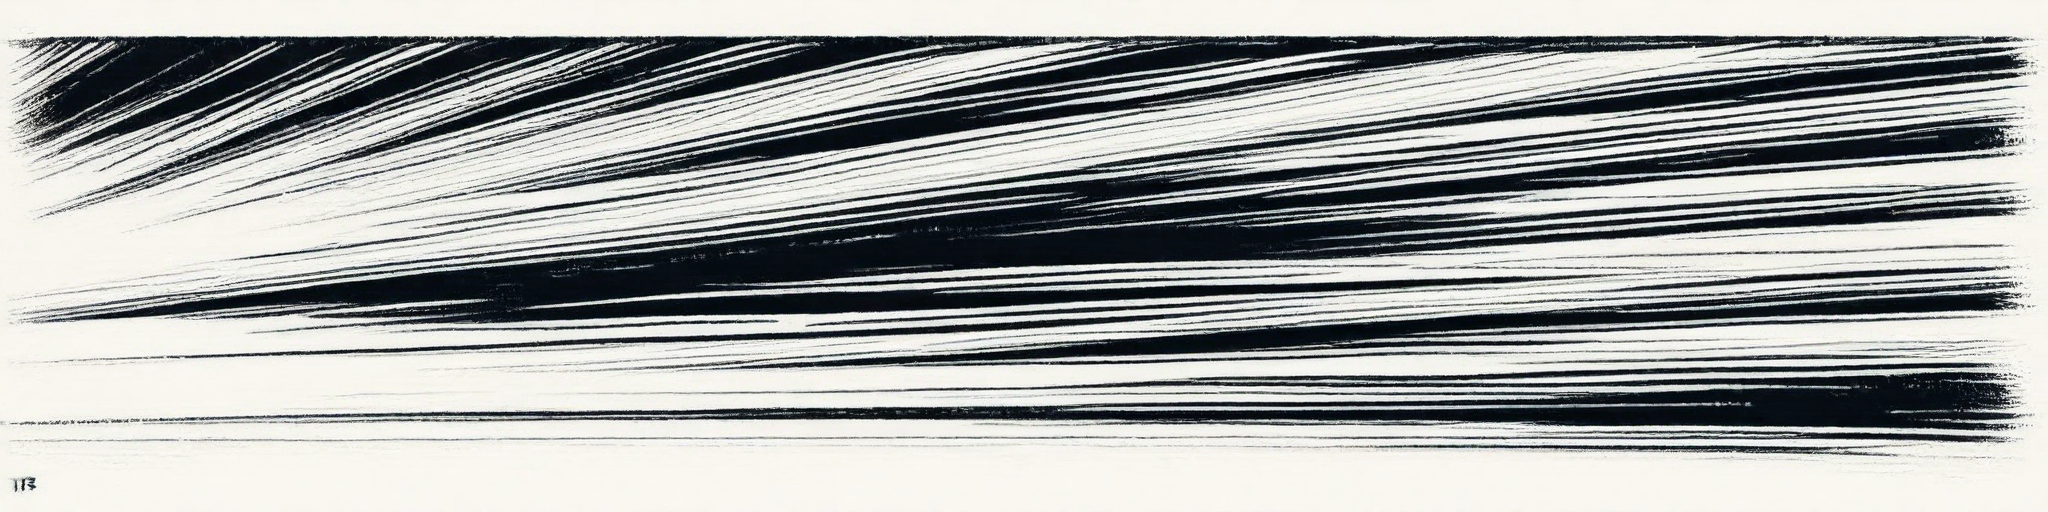
\includegraphics[width=\textwidth]{images/chapterImages/genesis_sketch_00119_.png}
\end{center}

Sarah woke at 3:17 AM with blueprints in her head.

Not metaphorical blueprints. Actual technical schematics. Satellite designs. Gravitational field generators. Orbital mechanics calculations. Knowledge she didn't have yesterday flooding in complete and perfect. She could see the entire defense grid. How it would deploy. How the satellites would coordinate. How the gravitational manipulation would work.

She reached for her laptop. Had to capture this. Had to record it before it faded.

It didn't fade. Just kept coming. More details. More systems. More understanding.

By 5 AM she'd filled forty pages of notes and the information was still flowing. Her hands were cramping. Eyes burning. Didn't matter. Had to get this down. Had to document everything.

By 7 AM she'd forgotten she'd meant to sleep. Food didn't occur to her. Shower didn't occur to her. Just the work. Just the relentless flood of understanding that needed to be captured, analyzed, implemented.

This was activation. This was what Marcus had been experiencing. This was the compulsion made real.

And it felt amazing.

That was the worst part. It felt right. Felt like coming home. Like finally understanding her purpose. Every discovery she'd ever made, every research breakthrough, every moment of scientific satisfaction—all of it was nothing compared to this. This was fulfillment. This was meaning. This was what she was designed to feel.

Like the first time she'd understood calculus, but more primal. Like the pull she'd felt at sixteen staring at equations until 4 AM, knowing her mother was worried but unable to stop. That same hunger, but infinite.

Her phone rang. She ignored it. Rang again. Again. Finally she picked up without checking who.

"What?"

"Sarah, it's Tom. Where are you? You missed the department meeting."

Tom. Her colleague. The meeting. She'd completely forgotten.

"I'm home. Working on something. Can't talk."

"Sarah, you're up for tenure review next month. You can't just skip—"

She hung up. Put the phone on silent. Turned back to her laptop.

The designs were more important than tenure. More important than her career. More important than everything.

By noon she'd contacted three aerospace engineers. Sent them partial designs. Waited for responses. They came back within hours—all confused, all intrigued, all asking the same question: How did you design this?

She didn't know how to answer. "Genetic activation" sounded insane. But it was the truth.

The responses kept coming. Engineers she'd sent designs to were sending modifications. Improvements. Additional systems. All of them spontaneous. All of them brilliant. All of them seemingly coming from nowhere.

The collective activation was happening. Thousands of people simultaneously receiving the same knowledge. The same capability. The same compulsion.

It was both terrifying and exhilarating.

Sarah's phone buzzed. Multiple messages. She glanced at them.

Tom: *Sarah, you need to call me. The dean wants to talk.*

Her ex: *You're late for Maya's birthday party. Where are you?*

She looked at the clock. 4:47 PM.

Maya's birthday.

Oh god. Maya's birthday.

She'd completely forgotten.

Sarah grabbed her keys. Ran to her car. Drove to Tom's house—her ex's house now. The house Maya lived in. The house Sarah visited twice a month if she remembered.

She arrived at 5:23. Cars in the driveway. Balloons on the mailbox. Party sounds from the backyard.

Sarah went around to the back gate. Found the celebration. Twenty kids. Parents. Cake. Maya in the center wearing a princess dress looking so happy.

Until she saw Sarah. Then the happiness drained. Replaced by something worse than anger. Resignation. Like Maya had learned not to expect anything and wasn't even disappointed anymore.

Tom saw her. His expression went cold.

"You're late."

"I'm sorry. I was working. I forgot—"

"You forgot your daughter's birthday."

The words hit like a physical blow. Sarah had forgotten Maya's birthday. Her eight-year-old daughter. The most important person in her life.

Except Maya wasn't the most important anymore. The work was more important. The compulsion made the work more important than everything.

For the work. For something she couldn't not do.

How many artists had said the same thing? How many musicians missed their children's recitals for one more session? How many writers chose the manuscript over the marriage? She'd judged them. Thought they were selfish. Thought they chose wrong.

Now she understood. They hadn't chosen at all.

"Maya, baby, I'm so sorry." Sarah approached. Tried to hug her daughter.

Maya stepped back. "You always say you're sorry."

"I know. I am. I brought your present—" Sarah hadn't brought the present. It was at home. Unwrapped. "—I'll give it to you later. Happy birthday, sweetie."

"I don't want a present."

"Maya—"

"I want you to remember. I want you to care. I want you to be my mom."

Sarah felt tears starting. "I am your mom. I do care. I just—"

"You were working. You're always working. You didn't come to my recital. You didn't come to my soccer game. You forgot my birthday. You don't love me anymore."

"That's not true. I love you so much."

"Then why don't you show it?"

Sarah didn't have an answer. Because the compulsion was stronger than love? Because she was genetically programmed to prioritize the work? Because her brain chemistry had been hijacked by activation sequences? None of that meant anything to an eight-year-old whose mother kept disappointing her.

Tom stepped in. "Maybe you should go, Sarah."

"I just got here—"

"And you're upsetting Maya. On her birthday. Which you forgot. Just... go. We'll talk later."

"I want to stay. I want to be here for—"

"Sarah." Tom's voice was quiet. Tired. "Look at yourself. When was the last time you slept? When was the last time you ate? You look like you're having a breakdown. Maya doesn't need to see you like this."

Sarah looked at her daughter. Maya was crying now. Quiet tears. Not dramatic. Just sad. Resigned to having a mother who didn't show up.

"I'm sorry," Sarah said again. Useless words. Empty words. "I'll make it up to you. I promise."

"You always promise," Maya said. "You never do."

Sarah left. Walked back to her car. Sat in the driver's seat with her hands shaking and tears running down her face.

She should stay. Should go back. Should fix this. Should prioritize her daughter over work.

But she could feel it. The compulsion. Pulling her attention back to the laptop. Back to the designs. Back to the work that provided relief from this emotional pain. The work that made sense. The work that was clear and purposeful and satisfying in ways parenting never was.

She started the car. Drove home. Opened her laptop. The designs were still there. Still demanding attention.

Sarah worked until 3 AM. Forgot about Maya's birthday. Forgot about her own failure. Forgot about everything except the defense grid.

The compulsion provided relief. Made the guilt manageable. Made the shame distant. Made everything except the work feel less real.

By morning, Maya's birthday was just a fact. A thing that had happened. Sarah felt bad about it. Would feel bad about it forever probably. But the badness was abstract. Intellectual. Not visceral anymore.

The compulsion had anesthetized her emotions. Made her effective. Made her functional. Made her into exactly the tool she was designed to be.

And she hated it.

And she couldn't stop it.

And she kept working anyway.

\scenebreak

Across the country, Marcus Chen hadn't come home in three days.

David found him in a rented warehouse in Oakland. Surrounded by equipment. Prototypes. Failed designs. Successful designs. Evidence of obsessive work at the expense of everything else.

"Marcus."

Marcus didn't look up. Was welding something. Sparks flying. Focus absolute.

"Marcus!"

He pulled off his welding mask. Looked at David like he was trying to remember who David was. Then recognition. "Hey. What time is it?"

"It's 4 AM. You didn't come home. You didn't call. I've been texting for two days. I thought you were dead."

"Sorry. I've been busy."

"Busy." David's voice was flat. "You've been busy. For three days. Without contacting me. Without telling me where you were. Without living in our apartment anymore apparently."

"I told you. The activation—"

"The activation. Right. The genetic compulsion. The thing you can't control." David moved closer. Saw the work space. The designs. The evidence of sophisticated engineering that Marcus shouldn't have been capable of. "What is all this?"

"Defense grid components. Gravitational manipulation systems. Orbital mechanics designs. I know how to build it, David. All of it. I can see exactly how it works."

"You're a mechanical engineer. You design industrial equipment."

"I was a mechanical engineer. Now I'm..." Marcus trailed off. Looked at his hands. "I don't know what I am now."

"You're my husband. Or you were. I'm not sure anymore."

Marcus set down his tools. Finally gave David his full attention. "I'm sorry. I know this is hard. I'm trying to—"

"You're not trying. You're completely consumed. You don't eat unless I remind you. You don't sleep unless you collapse. You don't talk unless I force you. You've disappeared into this work and I don't know how to get you back."

"I don't want to come back."

The words hung in the warehouse. Honest. Terrible. True.

David's expression cracked. "What?"

"I don't want to stop. I don't want to focus on anything else. This is the most important thing I've ever done. The most meaningful. The most right. And yes, it's programmed. Yes, it's activation. But it's still how I feel. The compulsion doesn't feel like slavery. It feels like purpose."

"More purpose than our relationship?"

"I don't know. Maybe. I'm sorry. But I can't lie to you. Can't pretend this isn't what I want even if wanting it is programmed."

David sat down on a crate. Looked at Marcus like seeing him for the first time. "Who are you?"

"I'm still Marcus."

"Are you? The Marcus I married wanted kids. Wanted to travel. Wanted to build furniture for our home and cook dinners and have conversations about books and movies. This person—" David gestured at the warehouse. "This person is a stranger. This person is obsessed. This person abandoned our life to build satellite components in a warehouse."

"The asteroid is real, David. If we don't build this defense grid, civilization ends. Billions of people die. Our future kids die. Everything dies. How do I choose our relationship over preventing that?"

"By being human. By recognizing that you're a person, not a tool. By exercising free will."

"What if I don't have free will? What if this compulsion is stronger than choice? What if I'm just code executing?"

"Then you're not responsible for abandoning me. But you're also not a person. You're just a program. And I can't be married to a program."

Marcus wanted to argue. Wanted to prove he was still himself. Still capable of love. Still choosing David despite the compulsion.

But he couldn't. The compulsion was always there. Always pulling. The moment this conversation ended, he'd go back to work. He knew it. David knew it. The relationship was already over. Just neither of them had acknowledged it yet.

"I'm sorry," Marcus said. "I love you. That's real. But I can't be what you need anymore."

"Can't or won't?"

"I don't know the difference."

David stood. "I'm leaving. Moving back to my sister's place in Portland. I'll get the rest of my stuff next week. I'll file the divorce papers. You... do whatever you're programmed to do."

"David—"

"Don't. Don't apologize again. Don't tell me you love me while choosing the work. Don't insult me by pretending you're trying."

He left. Marcus watched him go. Felt something break inside. Grief. Loss. The end of everything personal and private and beautiful they'd built together.

And underneath the grief: relief. Relief that he didn't have to balance anymore. Didn't have to pretend the relationship was as important as the work. Could fully commit to the compulsion without guilt.

The relief made him hate himself. But he turned back to his welding anyway.

The work demanded attention. The work provided satisfaction. The work was what he was designed to do.

David was right. Marcus wasn't a person anymore. Was just code executing. Just purpose. Just tool.

And he couldn't bring himself to care enough to fight it.

The compulsion had won.

\scenebreak

Around the world, the pattern repeated. Activated individuals abandoning relationships. Quitting jobs. Leaving lives. All driven by the same irresistible need to build.

Social media filled with confused posts. People describing the same symptoms. The intrusive knowledge. The compulsion. The inability to focus on anything except the work. Support groups formed. Forums emerged. People trying to understand what was happening to them.

And slowly, the realization spread: this was real. This was widespread. This was activation.

The secret couldn't hold. Too many people experiencing the same thing. Too many unexplainable capabilities emerging simultaneously. Too many brilliant designs coming from people who shouldn't have the knowledge to create them.

The media started reporting. At first skeptically. Then with growing concern. Then with something approaching panic. Thousands of engineers and physicists were experiencing simultaneous compulsion to build the same defense system. All claiming genetic programming. All showing evidence of capabilities beyond their training.

Either mass delusion or something unprecedented happening to human consciousness.

Governments got involved. Researchers like Sarah were contacted. Asked to explain. Asked to verify. Asked to help make sense of what was clearly happening but shouldn't be possible.

Sarah explained. Showed the genetic data. Demonstrated the correlation. Proved that activation sequences were expressing exactly on schedule.

The evidence was undeniable. Humanity was programmed. The activation was real. The compulsion was biological. And thousands of people were being transformed into something they hadn't chosen to become.

The philosophical implications could wait. The immediate concern was: what were all these activated people building? And should anyone try to stop them?

Sarah's answer was simple: They're building planetary defense. Against a real asteroid. On a real timeline. Stopping them means accepting extinction. Letting them continue means surrendering autonomy. There's no good option. Just necessary action.

The world chose necessity. Governments provided resources. Facilities. Coordination. The activated individuals self-organized. Built networks. Shared designs. Worked with collective purpose toward the same goal.

A global defense grid emerging from coordinated compulsion. Humanity working together not by choice but by programming. Building their salvation through the loss of free will.

And Sarah Chen, having missed her daughter's birthday to document activation, watched it all unfold with guilt and fascination and the growing certainty that she'd lost Maya forever.

The work continued.

The compulsion intensified.

The relationships fractured.

And the program executed regardless of cost.

Because that's what programs do. They execute. Regardless. Always. Without mercy.

The equation balanced.

The code ran.

The defense built itself.

And the people who were building it slowly stopped being people.

Became tools instead.

Conscious tools. Aware tools. Tools that suffered.

But tools nonetheless.

The activation was complete.

The transformation irreversible.

The purpose absolute.

And nothing—not love, not guilt, not the desperate need to be human—could stop it.

